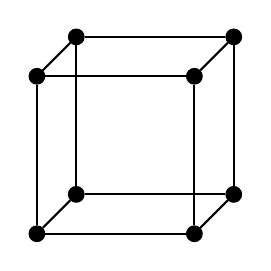
\begin{tikzpicture}
    [nodeDecorate/.style={inner sep=2pt,circle,draw=black,fill=black},%
        lineDecorate/.style={-,thick}]
    %% nodes or vertices
    \foreach \nodename/\x/\y in {
            1/0/0, 2/2/0, 3/2/2, 4/0/2, 5/0.5/0.5, 6/2.5/0.5, 7/2.5/2.5, 8/0.5/2.5}
        {
            \node (\nodename) at (\x,\y) [nodeDecorate] {};
        }
    %% edges or lines
    \path
    \foreach \startnode/\endnode in {
            1/2, 2/3, 3/4, 4/1, 5/6, 6/7, 7/8, 8/5, 1/5, 2/6, 3/7, 4/8}
        {
            (\startnode) edge[lineDecorate] node {} (\endnode)
        };
\end{tikzpicture}